% fig_mg_integration_scenario.tex
% TR-42: Scenario matrix outcome visualisation (10 scenarios)
% Fully hardcoded — no pgf math string comparisons

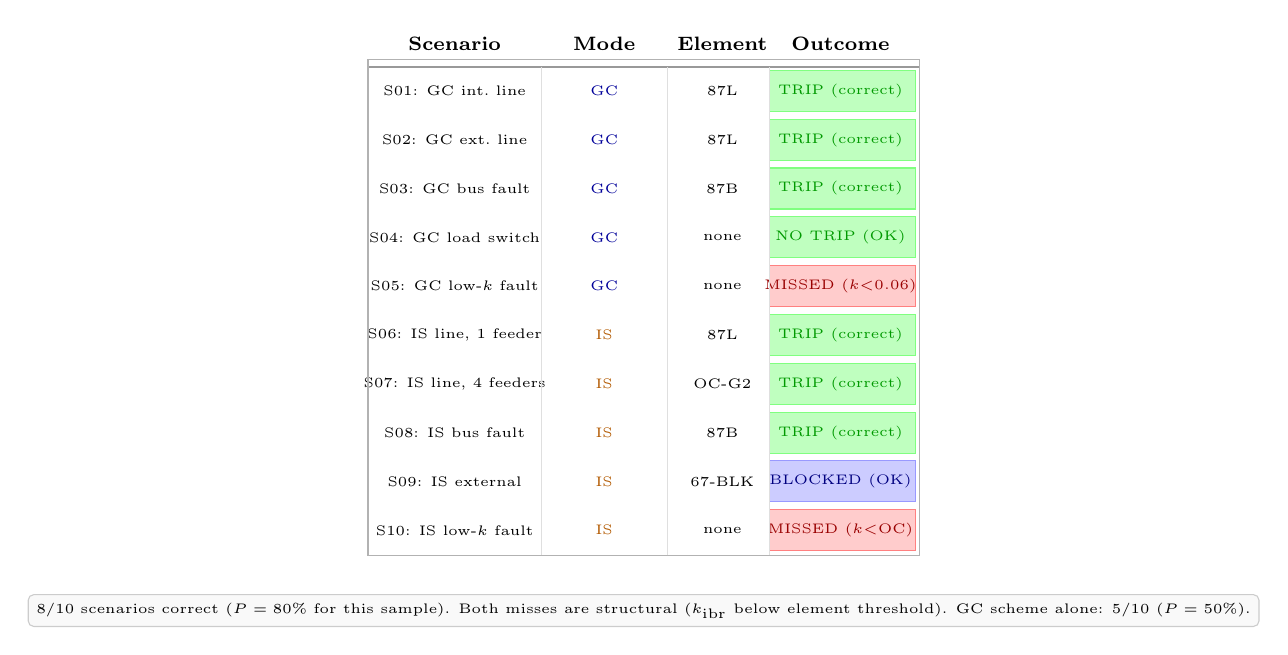
\begin{tikzpicture}[
  every node/.style={font=\tiny},
  cell/.style={minimum width=1.20cm, minimum height=0.55cm, align=center},
]

%% ── Column headers ─────────────────────────────────────────────────────────
\node[font=\scriptsize\bfseries] at (1.1, 5.70) {Scenario};
\node[font=\scriptsize\bfseries] at (3.0, 5.70) {Mode};
\node[font=\scriptsize\bfseries] at (4.5, 5.70) {Element};
\node[font=\scriptsize\bfseries, align=center] at (6.0, 5.70) {Outcome};
\draw[gray!80, thick] (0.0, 5.40) -- (7.0, 5.40);

%% ── Helper macro: draw one row ──────────────────────────────────────────────
%% \drawrow{y}{label}{mode}{modecol}{element}{fillcol}{bordervcol}{statustext}

%% Row 9 — S01
\node[align=left, font=\tiny] at (1.1, 5.10) {S01: GC int.\ line};
\node[font=\tiny, blue!60!black] at (3.0, 5.10) {GC};
\node[font=\tiny] at (4.5, 5.10) {87L};
\fill[green!25] (5.1, 4.84) rectangle (6.95, 5.36);
\draw[green!50, thin] (5.1, 4.84) rectangle (6.95, 5.36);
\node[font=\tiny, green!60!black] at (6.0, 5.10) {TRIP (correct)};

%% Row 8 — S02
\node[align=left] at (1.1, 4.48) {S02: GC ext.\ line};
\node[blue!60!black] at (3.0, 4.48) {GC};
\node at (4.5, 4.48) {87L};
\fill[green!25] (5.1, 4.22) rectangle (6.95, 4.74);
\draw[green!50, thin] (5.1, 4.22) rectangle (6.95, 4.74);
\node[green!60!black] at (6.0, 4.48) {TRIP (correct)};

%% Row 7 — S03
\node[align=left] at (1.1, 3.86) {S03: GC bus fault};
\node[blue!60!black] at (3.0, 3.86) {GC};
\node at (4.5, 3.86) {87B};
\fill[green!25] (5.1, 3.60) rectangle (6.95, 4.12);
\draw[green!50, thin] (5.1, 3.60) rectangle (6.95, 4.12);
\node[green!60!black] at (6.0, 3.86) {TRIP (correct)};

%% Row 6 — S04
\node[align=left] at (1.1, 3.24) {S04: GC load switch};
\node[blue!60!black] at (3.0, 3.24) {GC};
\node at (4.5, 3.24) {none};
\fill[green!25] (5.1, 2.98) rectangle (6.95, 3.50);
\draw[green!50, thin] (5.1, 2.98) rectangle (6.95, 3.50);
\node[green!60!black] at (6.0, 3.24) {NO TRIP (OK)};

%% Row 5 — S05 (MISSED)
\node[align=left] at (1.1, 2.62) {S05: GC low-$k$ fault};
\node[blue!60!black] at (3.0, 2.62) {GC};
\node at (4.5, 2.62) {none};
\fill[red!20] (5.1, 2.36) rectangle (6.95, 2.88);
\draw[red!50, thin] (5.1, 2.36) rectangle (6.95, 2.88);
\node[red!60!black] at (6.0, 2.62) {MISSED ($k{<}0.06$)};

%% Row 4 — S06
\node[align=left] at (1.1, 2.00) {S06: IS line, 1 feeder};
\node[orange!70!black] at (3.0, 2.00) {IS};
\node at (4.5, 2.00) {87L};
\fill[green!25] (5.1, 1.74) rectangle (6.95, 2.26);
\draw[green!50, thin] (5.1, 1.74) rectangle (6.95, 2.26);
\node[green!60!black] at (6.0, 2.00) {TRIP (correct)};

%% Row 3 — S07
\node[align=left] at (1.1, 1.38) {S07: IS line, 4 feeders};
\node[orange!70!black] at (3.0, 1.38) {IS};
\node at (4.5, 1.38) {OC-G2};
\fill[green!25] (5.1, 1.12) rectangle (6.95, 1.64);
\draw[green!50, thin] (5.1, 1.12) rectangle (6.95, 1.64);
\node[green!60!black] at (6.0, 1.38) {TRIP (correct)};

%% Row 2 — S08
\node[align=left] at (1.1, 0.76) {S08: IS bus fault};
\node[orange!70!black] at (3.0, 0.76) {IS};
\node at (4.5, 0.76) {87B};
\fill[green!25] (5.1, 0.50) rectangle (6.95, 1.02);
\draw[green!50, thin] (5.1, 0.50) rectangle (6.95, 1.02);
\node[green!60!black] at (6.0, 0.76) {TRIP (correct)};

%% Row 1 — S09 (external blocked)
\node[align=left] at (1.1, 0.14) {S09: IS external};
\node[orange!70!black] at (3.0, 0.14) {IS};
\node at (4.5, 0.14) {67-BLK};
\fill[blue!20] (5.1, -0.12) rectangle (6.95, 0.40);
\draw[blue!40, thin] (5.1, -0.12) rectangle (6.95, 0.40);
\node[blue!50!black] at (6.0, 0.14) {BLOCKED (OK)};

%% Row 0 — S10 (MISSED)
\node[align=left] at (1.1, -0.48) {S10: IS low-$k$ fault};
\node[orange!70!black] at (3.0, -0.48) {IS};
\node at (4.5, -0.48) {none};
\fill[red!20] (5.1, -0.74) rectangle (6.95, -0.22);
\draw[red!50, thin] (5.1, -0.74) rectangle (6.95, -0.22);
\node[red!60!black] at (6.0, -0.48) {MISSED ($k{<}$OC)};

%% Outer border and column separators
\draw[gray!60, thin] (0.0, -0.80) rectangle (7.0, 5.50);
\foreach \x in {2.2, 3.8, 5.1} {
  \draw[gray!25, thin] (\x, -0.80) -- (\x, 5.40);
}

%% Summary annotation
\node[draw=gray!40, fill=gray!5, rounded corners=2pt,
      font=\tiny, inner sep=3pt, align=center]
  at (3.5, -1.50)
  {8/10 scenarios correct ($P=80\%$ for this sample).
   Both misses are structural ($k_\mathrm{ibr}$ below element threshold).
   GC scheme alone: 5/10 ($P=50\%$).};

\end{tikzpicture}
